\documentclass[twoside]{book}

% Packages required by doxygen
\usepackage{fixltx2e}
\usepackage{calc}
\usepackage{doxygen}
\usepackage{graphicx}
\usepackage[utf8]{inputenc}
\usepackage{makeidx}
\usepackage{multicol}
\usepackage{multirow}
\PassOptionsToPackage{warn}{textcomp}
\usepackage{textcomp}
\usepackage[nointegrals]{wasysym}
\usepackage[table]{xcolor}

% Font selection
\usepackage[T1]{fontenc}
\usepackage{mathptmx}
\usepackage[scaled=.90]{helvet}
\usepackage{courier}
\usepackage{amssymb}
\usepackage{sectsty}
\renewcommand{\familydefault}{\sfdefault}
\allsectionsfont{%
  \fontseries{bc}\selectfont%
  \color{darkgray}%
}
\renewcommand{\DoxyLabelFont}{%
  \fontseries{bc}\selectfont%
  \color{darkgray}%
}
\newcommand{\+}{\discretionary{\mbox{\scriptsize$\hookleftarrow$}}{}{}}

% Page & text layout
\usepackage{geometry}
\geometry{%
  a4paper,%
  top=2.5cm,%
  bottom=2.5cm,%
  left=2.5cm,%
  right=2.5cm%
}
\tolerance=750
\hfuzz=15pt
\hbadness=750
\setlength{\emergencystretch}{15pt}
\setlength{\parindent}{0cm}
\setlength{\parskip}{0.2cm}
\makeatletter
\renewcommand{\paragraph}{%
  \@startsection{paragraph}{4}{0ex}{-1.0ex}{1.0ex}{%
    \normalfont\normalsize\bfseries\SS@parafont%
  }%
}
\renewcommand{\subparagraph}{%
  \@startsection{subparagraph}{5}{0ex}{-1.0ex}{1.0ex}{%
    \normalfont\normalsize\bfseries\SS@subparafont%
  }%
}
\makeatother

% Headers & footers
\usepackage{fancyhdr}
\pagestyle{fancyplain}
\fancyhead[LE]{\fancyplain{}{\bfseries\thepage}}
\fancyhead[CE]{\fancyplain{}{}}
\fancyhead[RE]{\fancyplain{}{\bfseries\leftmark}}
\fancyhead[LO]{\fancyplain{}{\bfseries\rightmark}}
\fancyhead[CO]{\fancyplain{}{}}
\fancyhead[RO]{\fancyplain{}{\bfseries\thepage}}
\fancyfoot[LE]{\fancyplain{}{}}
\fancyfoot[CE]{\fancyplain{}{}}
\fancyfoot[RE]{\fancyplain{}{\bfseries\scriptsize Generated on Tue Dec 11 2018 17\+:22\+:08 for vmsim by Doxygen }}
\fancyfoot[LO]{\fancyplain{}{\bfseries\scriptsize Generated on Tue Dec 11 2018 17\+:22\+:08 for vmsim by Doxygen }}
\fancyfoot[CO]{\fancyplain{}{}}
\fancyfoot[RO]{\fancyplain{}{}}
\renewcommand{\footrulewidth}{0.4pt}
\renewcommand{\chaptermark}[1]{%
  \markboth{#1}{}%
}
\renewcommand{\sectionmark}[1]{%
  \markright{\thesection\ #1}%
}

% Indices & bibliography
\usepackage{natbib}
\usepackage[titles]{tocloft}
\setcounter{tocdepth}{3}
\setcounter{secnumdepth}{5}
\makeindex

% Hyperlinks (required, but should be loaded last)
\usepackage{ifpdf}
\ifpdf
  \usepackage[pdftex,pagebackref=true]{hyperref}
\else
  \usepackage[ps2pdf,pagebackref=true]{hyperref}
\fi
\hypersetup{%
  colorlinks=true,%
  linkcolor=blue,%
  citecolor=blue,%
  unicode%
}

% Custom commands
\newcommand{\clearemptydoublepage}{%
  \newpage{\pagestyle{empty}\cleardoublepage}%
}


%===== C O N T E N T S =====

\begin{document}

% Titlepage & ToC
\hypersetup{pageanchor=false,
             bookmarks=true,
             bookmarksnumbered=true,
             pdfencoding=unicode
            }
\pagenumbering{roman}
\begin{titlepage}
\vspace*{7cm}
\begin{center}%
{\Large vmsim \\[1ex]\large project-\/4 }\\
\vspace*{1cm}
{\large Generated by Doxygen 1.8.7}\\
\vspace*{0.5cm}
{\small Tue Dec 11 2018 17:22:08}\\
\end{center}
\end{titlepage}
\clearemptydoublepage
\tableofcontents
\clearemptydoublepage
\pagenumbering{arabic}
\hypersetup{pageanchor=true}

%--- Begin generated contents ---
\chapter{File Index}
\section{File List}
Here is a list of all documented files with brief descriptions\+:\begin{DoxyCompactList}
\item\contentsline{section}{\hyperlink{bs_8h}{bs.\+h} \\*The interface for the backing store device }{\pageref{bs_8h}}{}
\item\contentsline{section}{\hyperlink{iterative-walk_8c}{iterative-\/walk.\+c} \\*Create an array, and iterate over it. Use the {\ttfamily vmsim} library for the array }{\pageref{iterative-walk_8c}}{}
\item\contentsline{section}{\hyperlink{mmu_8h}{mmu.\+h} \\*The interface for the M\+M\+U module }{\pageref{mmu_8h}}{}
\item\contentsline{section}{\hyperlink{random-hop_8c}{random-\/hop.\+c} \\*Within a simulated space, jump randomly to locations, marking each and ending when a location is revisited }{\pageref{random-hop_8c}}{}
\item\contentsline{section}{\hyperlink{vmsim_8h}{vmsim.\+h} \\*The interface for the {\ttfamily vmsim} library }{\pageref{vmsim_8h}}{}
\end{DoxyCompactList}

\chapter{File Documentation}
\hypertarget{bs_8h}{\section{bs.\+h File Reference}
\label{bs_8h}\index{bs.\+h@{bs.\+h}}
}


The interface for the backing store device.  


{\ttfamily \#include $<$stdbool.\+h$>$}\\*
{\ttfamily \#include $<$stdlib.\+h$>$}\\*
{\ttfamily \#include \char`\"{}vmsim.\+h\char`\"{}}\\*
Include dependency graph for bs.\+h\+:\nopagebreak
\begin{figure}[H]
\begin{center}
\leavevmode
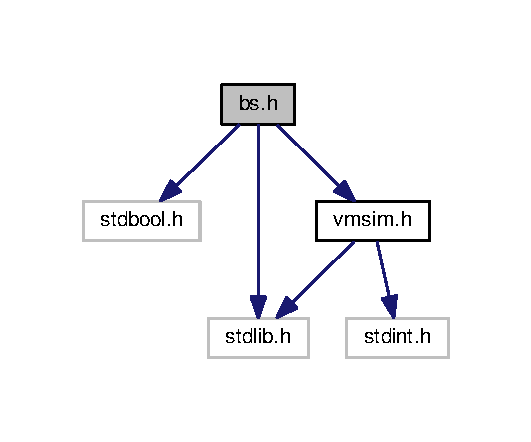
\includegraphics[width=255pt]{bs_8h__incl}
\end{center}
\end{figure}
\subsection*{Functions}
\begin{DoxyCompactItemize}
\item 
\hypertarget{bs_8h_a03018e086880812b45ca6612dd0d50fe}{void \hyperlink{bs_8h_a03018e086880812b45ca6612dd0d50fe}{bs\+\_\+init} ()}\label{bs_8h_a03018e086880812b45ca6612dd0d50fe}

\begin{DoxyCompactList}\small\item\em Initialize the simulated backing store device. \end{DoxyCompactList}\item 
bool \hyperlink{bs_8h_ac1ecd778f4899fecb6f736d83c3bb0ad}{bs\+\_\+read} (\hyperlink{vmsim_8h_a1ad4b372d1694c5c19ee7ccada09d807}{vmsim\+\_\+addr\+\_\+t} buffer, unsigned int block\+\_\+number)
\begin{DoxyCompactList}\small\item\em Read data from a block. \end{DoxyCompactList}\item 
bool \hyperlink{bs_8h_a377e509bff1a6c91f5eeb91623d449ca}{bs\+\_\+write} (\hyperlink{vmsim_8h_a1ad4b372d1694c5c19ee7ccada09d807}{vmsim\+\_\+addr\+\_\+t} buffer, unsigned int block\+\_\+number)
\begin{DoxyCompactList}\small\item\em Write data to a block. \end{DoxyCompactList}\end{DoxyCompactItemize}


\subsection{Detailed Description}
The interface for the backing store device. 

\begin{DoxyAuthor}{Author}
Prof. Scott F. Kaplan 
\end{DoxyAuthor}
\begin{DoxyDate}{Date}
Fall 2018 
\end{DoxyDate}


\subsection{Function Documentation}
\hypertarget{bs_8h_ac1ecd778f4899fecb6f736d83c3bb0ad}{\index{bs.\+h@{bs.\+h}!bs\+\_\+read@{bs\+\_\+read}}
\index{bs\+\_\+read@{bs\+\_\+read}!bs.\+h@{bs.\+h}}
\subsubsection[{bs\+\_\+read}]{\setlength{\rightskip}{0pt plus 5cm}bool bs\+\_\+read (
\begin{DoxyParamCaption}
\item[{{\bf vmsim\+\_\+addr\+\_\+t}}]{buffer, }
\item[{unsigned int}]{block\+\_\+number}
\end{DoxyParamCaption}
)}}\label{bs_8h_ac1ecd778f4899fecb6f736d83c3bb0ad}


Read data from a block. 


\begin{DoxyParams}{Parameters}
{\em buffer} & The {\itshape real} address of a space into which to copy the block's data. \\
\hline
{\em block\+\_\+number} & The block number of the backing store to read. \\
\hline
\end{DoxyParams}
\begin{DoxyReturn}{Returns}
whether the operation was successful. 
\end{DoxyReturn}
\hypertarget{bs_8h_a377e509bff1a6c91f5eeb91623d449ca}{\index{bs.\+h@{bs.\+h}!bs\+\_\+write@{bs\+\_\+write}}
\index{bs\+\_\+write@{bs\+\_\+write}!bs.\+h@{bs.\+h}}
\subsubsection[{bs\+\_\+write}]{\setlength{\rightskip}{0pt plus 5cm}bool bs\+\_\+write (
\begin{DoxyParamCaption}
\item[{{\bf vmsim\+\_\+addr\+\_\+t}}]{buffer, }
\item[{unsigned int}]{block\+\_\+number}
\end{DoxyParamCaption}
)}}\label{bs_8h_a377e509bff1a6c91f5eeb91623d449ca}


Write data to a block. 


\begin{DoxyParams}{Parameters}
{\em buffer} & The {\itshape real} address of a space from which to copy the block's data. \\
\hline
{\em block\+\_\+number} & The block number of the backing store to write. \\
\hline
\end{DoxyParams}
\begin{DoxyReturn}{Returns}
whether the operation was successful. 
\end{DoxyReturn}

\hypertarget{iterative-walk_8c}{\section{iterative-\/walk.c File Reference}
\label{iterative-walk_8c}\index{iterative-\/walk.\+c@{iterative-\/walk.\+c}}
}


Create an array, and iterate over it. Use the {\ttfamily vmsim} library for the array.  


{\ttfamily \#include $<$assert.\+h$>$}\\*
{\ttfamily \#include $<$errno.\+h$>$}\\*
{\ttfamily \#include $<$stdbool.\+h$>$}\\*
{\ttfamily \#include $<$stdint.\+h$>$}\\*
{\ttfamily \#include $<$stdio.\+h$>$}\\*
{\ttfamily \#include $<$stdlib.\+h$>$}\\*
{\ttfamily \#include \char`\"{}vmsim.\+h\char`\"{}}\\*
Include dependency graph for iterative-\/walk.c\+:\nopagebreak
\begin{figure}[H]
\begin{center}
\leavevmode
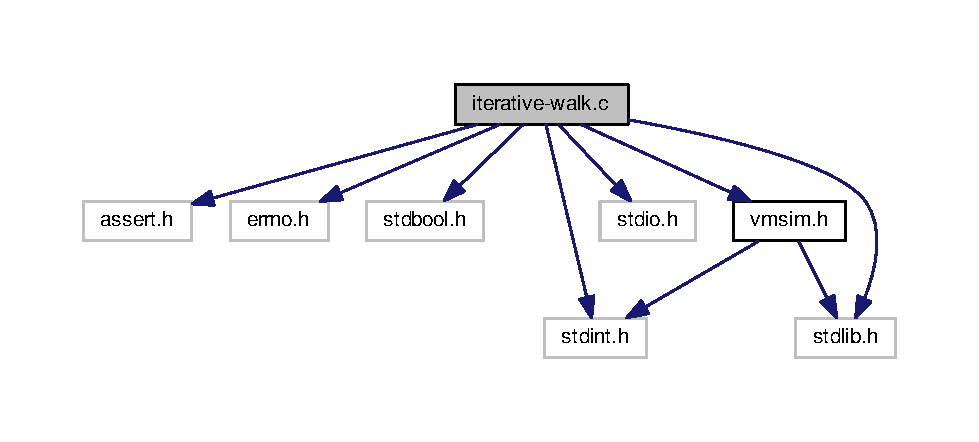
\includegraphics[width=350pt]{iterative-walk_8c__incl}
\end{center}
\end{figure}
\subsection*{Macros}
\begin{DoxyCompactItemize}
\item 
\#define \hyperlink{iterative-walk_8c_ab5fde4a4261bca6820d8cd5b0d3a1b8d}{B\+Y\+T\+E\+S\+\_\+\+P\+E\+R\+\_\+\+K\+B}~1024
\end{DoxyCompactItemize}
\subsection*{Functions}
\begin{DoxyCompactItemize}
\item 
void \hyperlink{iterative-walk_8c_a4c03bd347423374d85d921056bd14e5c}{show\+\_\+usage\+\_\+and\+\_\+exit} (char $\ast$invocation)
\begin{DoxyCompactList}\small\item\em Display the proper usage and end the process with an error code. \end{DoxyCompactList}\item 
void \hyperlink{iterative-walk_8c_a92da6e3eac55a76919d70a529698cba3}{populate} (\hyperlink{vmsim_8h_a1ad4b372d1694c5c19ee7ccada09d807}{vmsim\+\_\+addr\+\_\+t} array, unsigned int length)
\begin{DoxyCompactList}\small\item\em Initialize an array with values such that each entry contains its own index. \end{DoxyCompactList}\item 
void \hyperlink{iterative-walk_8c_a8934a56f7be8726dbed732e41a1639ed}{traverse} (\hyperlink{vmsim_8h_a1ad4b372d1694c5c19ee7ccada09d807}{vmsim\+\_\+addr\+\_\+t} array, unsigned int length)
\begin{DoxyCompactList}\small\item\em Move through the array, summing the values found and storing the running sum into each position. \end{DoxyCompactList}\item 
void \hyperlink{iterative-walk_8c_a2e85b0f86f91c0581fcd8e5bd6764568}{go} (unsigned int length, unsigned int iterations)
\begin{DoxyCompactList}\small\item\em Create an array, initiialize it, and then traverse it repeatedly. \end{DoxyCompactList}\item 
int \hyperlink{iterative-walk_8c_a3c04138a5bfe5d72780bb7e82a18e627}{main} (int argc, char $\ast$$\ast$argv)
\begin{DoxyCompactList}\small\item\em The entry point to the simulator. \end{DoxyCompactList}\end{DoxyCompactItemize}


\subsection{Detailed Description}
Create an array, and iterate over it. Use the {\ttfamily vmsim} library for the array. 

\begin{DoxyAuthor}{Author}
Prof. Scott F. Kaplan 
\end{DoxyAuthor}
\begin{DoxyDate}{Date}
Fall 2018 
\end{DoxyDate}


\subsection{Macro Definition Documentation}
\hypertarget{iterative-walk_8c_ab5fde4a4261bca6820d8cd5b0d3a1b8d}{\index{iterative-\/walk.\+c@{iterative-\/walk.\+c}!B\+Y\+T\+E\+S\+\_\+\+P\+E\+R\+\_\+\+K\+B@{B\+Y\+T\+E\+S\+\_\+\+P\+E\+R\+\_\+\+K\+B}}
\index{B\+Y\+T\+E\+S\+\_\+\+P\+E\+R\+\_\+\+K\+B@{B\+Y\+T\+E\+S\+\_\+\+P\+E\+R\+\_\+\+K\+B}!iterative-\/walk.\+c@{iterative-\/walk.\+c}}
\subsubsection[{B\+Y\+T\+E\+S\+\_\+\+P\+E\+R\+\_\+\+K\+B}]{\setlength{\rightskip}{0pt plus 5cm}\#define B\+Y\+T\+E\+S\+\_\+\+P\+E\+R\+\_\+\+K\+B~1024}}\label{iterative-walk_8c_ab5fde4a4261bca6820d8cd5b0d3a1b8d}
The number of bytes in an kilobyte. 

\subsection{Function Documentation}
\hypertarget{iterative-walk_8c_a2e85b0f86f91c0581fcd8e5bd6764568}{\index{iterative-\/walk.\+c@{iterative-\/walk.\+c}!go@{go}}
\index{go@{go}!iterative-\/walk.\+c@{iterative-\/walk.\+c}}
\subsubsection[{go}]{\setlength{\rightskip}{0pt plus 5cm}void go (
\begin{DoxyParamCaption}
\item[{unsigned int}]{length, }
\item[{unsigned int}]{iterations}
\end{DoxyParamCaption}
)}}\label{iterative-walk_8c_a2e85b0f86f91c0581fcd8e5bd6764568}


Create an array, initiialize it, and then traverse it repeatedly. 


\begin{DoxyParams}{Parameters}
{\em length} & The size of the array to create. \\
\hline
{\em iterations} & The number of traversals to perform on the array. \\
\hline
\end{DoxyParams}
\hypertarget{iterative-walk_8c_a3c04138a5bfe5d72780bb7e82a18e627}{\index{iterative-\/walk.\+c@{iterative-\/walk.\+c}!main@{main}}
\index{main@{main}!iterative-\/walk.\+c@{iterative-\/walk.\+c}}
\subsubsection[{main}]{\setlength{\rightskip}{0pt plus 5cm}int main (
\begin{DoxyParamCaption}
\item[{int}]{argc, }
\item[{char $\ast$$\ast$}]{argv}
\end{DoxyParamCaption}
)}}\label{iterative-walk_8c_a3c04138a5bfe5d72780bb7e82a18e627}


The entry point to the simulator. 


\begin{DoxyParams}{Parameters}
{\em argc} & The length of the command-\/line argument vector. \\
\hline
{\em argv} & The vector of command-\/line arguments. \\
\hline
\end{DoxyParams}
\begin{DoxyReturn}{Returns}
the exit code for the process, where 0 indicates success, any other value indicates error. 
\end{DoxyReturn}
\hypertarget{iterative-walk_8c_a92da6e3eac55a76919d70a529698cba3}{\index{iterative-\/walk.\+c@{iterative-\/walk.\+c}!populate@{populate}}
\index{populate@{populate}!iterative-\/walk.\+c@{iterative-\/walk.\+c}}
\subsubsection[{populate}]{\setlength{\rightskip}{0pt plus 5cm}void populate (
\begin{DoxyParamCaption}
\item[{{\bf vmsim\+\_\+addr\+\_\+t}}]{array, }
\item[{unsigned int}]{length}
\end{DoxyParamCaption}
)}}\label{iterative-walk_8c_a92da6e3eac55a76919d70a529698cba3}


Initialize an array with values such that each entry contains its own index. 


\begin{DoxyParams}{Parameters}
{\em array} & The simulated address of an array of unsigned 64-\/bit integers. \\
\hline
{\em length} & The number of elements in the array. \\
\hline
\end{DoxyParams}
\hypertarget{iterative-walk_8c_a4c03bd347423374d85d921056bd14e5c}{\index{iterative-\/walk.\+c@{iterative-\/walk.\+c}!show\+\_\+usage\+\_\+and\+\_\+exit@{show\+\_\+usage\+\_\+and\+\_\+exit}}
\index{show\+\_\+usage\+\_\+and\+\_\+exit@{show\+\_\+usage\+\_\+and\+\_\+exit}!iterative-\/walk.\+c@{iterative-\/walk.\+c}}
\subsubsection[{show\+\_\+usage\+\_\+and\+\_\+exit}]{\setlength{\rightskip}{0pt plus 5cm}void show\+\_\+usage\+\_\+and\+\_\+exit (
\begin{DoxyParamCaption}
\item[{char $\ast$}]{invocation}
\end{DoxyParamCaption}
)}}\label{iterative-walk_8c_a4c03bd347423374d85d921056bd14e5c}


Display the proper usage and end the process with an error code. 


\begin{DoxyParams}{Parameters}
{\em invocation} & The command-\/line text given to run the executable. \\
\hline
\end{DoxyParams}
\hypertarget{iterative-walk_8c_a8934a56f7be8726dbed732e41a1639ed}{\index{iterative-\/walk.\+c@{iterative-\/walk.\+c}!traverse@{traverse}}
\index{traverse@{traverse}!iterative-\/walk.\+c@{iterative-\/walk.\+c}}
\subsubsection[{traverse}]{\setlength{\rightskip}{0pt plus 5cm}void traverse (
\begin{DoxyParamCaption}
\item[{{\bf vmsim\+\_\+addr\+\_\+t}}]{array, }
\item[{unsigned int}]{length}
\end{DoxyParamCaption}
)}}\label{iterative-walk_8c_a8934a56f7be8726dbed732e41a1639ed}


Move through the array, summing the values found and storing the running sum into each position. 


\begin{DoxyParams}{Parameters}
{\em array} & The simulated address of an array of unsigned 64-\/bit integers. \\
\hline
{\em length} & The number of elements in the array. \\
\hline
\end{DoxyParams}

\hypertarget{mmu_8h}{\section{mmu.\+h File Reference}
\label{mmu_8h}\index{mmu.\+h@{mmu.\+h}}
}


The interface for the M\+M\+U module.  


{\ttfamily \#include $<$stdbool.\+h$>$}\\*
{\ttfamily \#include \char`\"{}vmsim.\+h\char`\"{}}\\*
Include dependency graph for mmu.\+h\+:\nopagebreak
\begin{figure}[H]
\begin{center}
\leavevmode
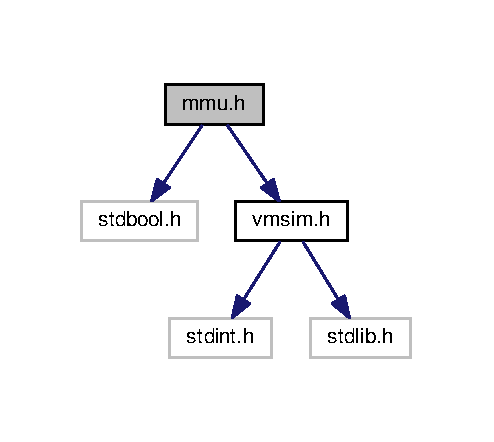
\includegraphics[width=237pt]{mmu_8h__incl}
\end{center}
\end{figure}
\subsection*{Functions}
\begin{DoxyCompactItemize}
\item 
void \hyperlink{mmu_8h_a8e19b138abc93c22f9669a284e2b6a2b}{mmu\+\_\+init} (\hyperlink{vmsim_8h_a1ad4b372d1694c5c19ee7ccada09d807}{vmsim\+\_\+addr\+\_\+t} upper\+\_\+pt\+\_\+addr)
\begin{DoxyCompactList}\small\item\em Initialize the M\+M\+U. \end{DoxyCompactList}\item 
\hyperlink{vmsim_8h_a1ad4b372d1694c5c19ee7ccada09d807}{vmsim\+\_\+addr\+\_\+t} \hyperlink{mmu_8h_aa419e279930d7e9d880947d03d92c8f9}{mmu\+\_\+translate} (\hyperlink{vmsim_8h_a1ad4b372d1694c5c19ee7ccada09d807}{vmsim\+\_\+addr\+\_\+t} sim\+\_\+addr, bool write\+\_\+operation)
\begin{DoxyCompactList}\small\item\em Translate a simulated address into a physical address. \end{DoxyCompactList}\end{DoxyCompactItemize}


\subsection{Detailed Description}
The interface for the M\+M\+U module. 

\begin{DoxyAuthor}{Author}
Prof. Scott F. Kaplan 
\end{DoxyAuthor}
\begin{DoxyDate}{Date}
Fall 2018
\end{DoxyDate}
A simple module that is part of the {\ttfamily vmsim} library. This module implements the simulated {\itshape memory management unit (M\+M\+U)} that typically provides hardware mapping of virtual-\/to-\/physical addresses. 

\subsection{Function Documentation}
\hypertarget{mmu_8h_a8e19b138abc93c22f9669a284e2b6a2b}{\index{mmu.\+h@{mmu.\+h}!mmu\+\_\+init@{mmu\+\_\+init}}
\index{mmu\+\_\+init@{mmu\+\_\+init}!mmu.\+h@{mmu.\+h}}
\subsubsection[{mmu\+\_\+init}]{\setlength{\rightskip}{0pt plus 5cm}void mmu\+\_\+init (
\begin{DoxyParamCaption}
\item[{{\bf vmsim\+\_\+addr\+\_\+t}}]{upper\+\_\+pt\+\_\+addr}
\end{DoxyParamCaption}
)}}\label{mmu_8h_a8e19b138abc93c22f9669a284e2b6a2b}


Initialize the M\+M\+U. 


\begin{DoxyParams}{Parameters}
{\em upper\+\_\+pt\+\_\+addr} & The real base address of the upper page table.\\
\hline
\end{DoxyParams}
This function stores the given real address of the upper page table. Doing so is analogous to setting a hardware M\+M\+U's {\itshape page table register (P\+T\+R)} with the physical base address of the upper P\+T. \hypertarget{mmu_8h_aa419e279930d7e9d880947d03d92c8f9}{\index{mmu.\+h@{mmu.\+h}!mmu\+\_\+translate@{mmu\+\_\+translate}}
\index{mmu\+\_\+translate@{mmu\+\_\+translate}!mmu.\+h@{mmu.\+h}}
\subsubsection[{mmu\+\_\+translate}]{\setlength{\rightskip}{0pt plus 5cm}{\bf vmsim\+\_\+addr\+\_\+t} mmu\+\_\+translate (
\begin{DoxyParamCaption}
\item[{{\bf vmsim\+\_\+addr\+\_\+t}}]{sim\+\_\+addr, }
\item[{bool}]{write\+\_\+operation}
\end{DoxyParamCaption}
)}}\label{mmu_8h_aa419e279930d7e9d880947d03d92c8f9}


Translate a simulated address into a physical address. 


\begin{DoxyParams}{Parameters}
{\em sim\+\_\+addr} & The simulated address to be translated. \\
\hline
{\em write\+\_\+operation} & Whether the data at the given address is being {\itshape read} ({\ttfamily false}) or {\itshape written} ({\ttfamily true}). \\
\hline
\end{DoxyParams}
\begin{DoxyReturn}{Returns}
the real address to which the simulated address maps.
\end{DoxyReturn}
This function walks the multi-\/level page table to find the mapping from the given simulated address to its corresponding real address. If the simulated address is not yet mapped to a real address, then this function calls {\ttfamily \hyperlink{vmsim_8h_a2f2b0d73cdb718c73fbf3046dcaec0ca}{vmsim\+\_\+map\+\_\+fault()}} (mimicking an {\itshape address translation interrupt}, or {\itshape page fault}, in hardware) to have the mapping created, and then restarts the translation. 
\hypertarget{random-hop_8c}{\section{random-\/hop.c File Reference}
\label{random-hop_8c}\index{random-\/hop.\+c@{random-\/hop.\+c}}
}


Within a simulated space, jump randomly to locations, marking each and ending when a location is revisited.  


{\ttfamily \#include $<$assert.\+h$>$}\\*
{\ttfamily \#include $<$errno.\+h$>$}\\*
{\ttfamily \#include $<$stdbool.\+h$>$}\\*
{\ttfamily \#include $<$stdint.\+h$>$}\\*
{\ttfamily \#include $<$stdio.\+h$>$}\\*
{\ttfamily \#include $<$stdlib.\+h$>$}\\*
{\ttfamily \#include \char`\"{}vmsim.\+h\char`\"{}}\\*
Include dependency graph for random-\/hop.c\+:\nopagebreak
\begin{figure}[H]
\begin{center}
\leavevmode
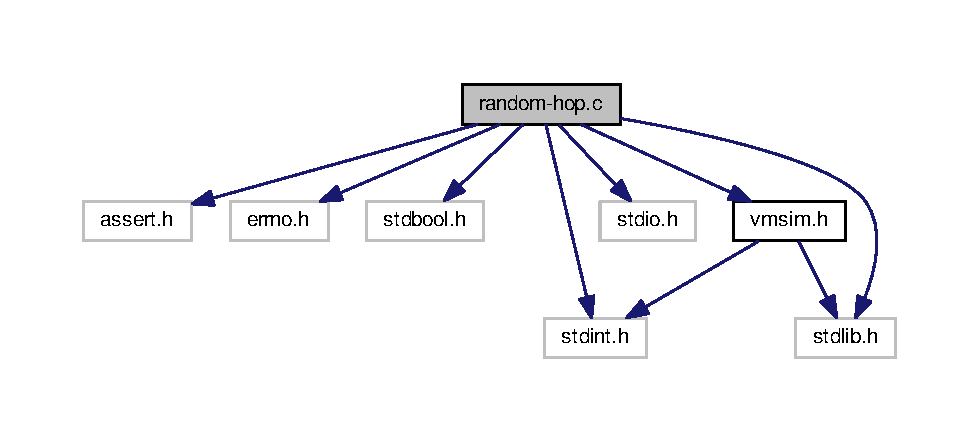
\includegraphics[width=350pt]{random-hop_8c__incl}
\end{center}
\end{figure}
\subsection*{Macros}
\begin{DoxyCompactItemize}
\item 
\#define \hyperlink{random-hop_8c_ab5fde4a4261bca6820d8cd5b0d3a1b8d}{B\+Y\+T\+E\+S\+\_\+\+P\+E\+R\+\_\+\+K\+B}~1024
\end{DoxyCompactItemize}
\subsection*{Functions}
\begin{DoxyCompactItemize}
\item 
void \hyperlink{random-hop_8c_a4c03bd347423374d85d921056bd14e5c}{show\+\_\+usage\+\_\+and\+\_\+exit} (char $\ast$invocation)
\begin{DoxyCompactList}\small\item\em Display the proper usage and end the process with an error code. \end{DoxyCompactList}\item 
void \hyperlink{random-hop_8c_a19ca1a272fed125876eb02b534d261f3}{go} (unsigned int size)
\begin{DoxyCompactList}\small\item\em Randomly visit simulated addresses, marking locations until an already-\/marked one is visited. \end{DoxyCompactList}\item 
int \hyperlink{random-hop_8c_a3c04138a5bfe5d72780bb7e82a18e627}{main} (int argc, char $\ast$$\ast$argv)
\begin{DoxyCompactList}\small\item\em The entry point to the simulator. \end{DoxyCompactList}\end{DoxyCompactItemize}


\subsection{Detailed Description}
Within a simulated space, jump randomly to locations, marking each and ending when a location is revisited. 

\begin{DoxyAuthor}{Author}
Prof. Scott F. Kaplan 
\end{DoxyAuthor}
\begin{DoxyDate}{Date}
Fall 2018 
\end{DoxyDate}


\subsection{Macro Definition Documentation}
\hypertarget{random-hop_8c_ab5fde4a4261bca6820d8cd5b0d3a1b8d}{\index{random-\/hop.\+c@{random-\/hop.\+c}!B\+Y\+T\+E\+S\+\_\+\+P\+E\+R\+\_\+\+K\+B@{B\+Y\+T\+E\+S\+\_\+\+P\+E\+R\+\_\+\+K\+B}}
\index{B\+Y\+T\+E\+S\+\_\+\+P\+E\+R\+\_\+\+K\+B@{B\+Y\+T\+E\+S\+\_\+\+P\+E\+R\+\_\+\+K\+B}!random-\/hop.\+c@{random-\/hop.\+c}}
\subsubsection[{B\+Y\+T\+E\+S\+\_\+\+P\+E\+R\+\_\+\+K\+B}]{\setlength{\rightskip}{0pt plus 5cm}\#define B\+Y\+T\+E\+S\+\_\+\+P\+E\+R\+\_\+\+K\+B~1024}}\label{random-hop_8c_ab5fde4a4261bca6820d8cd5b0d3a1b8d}
The number of bytes in an kilobyte. 

\subsection{Function Documentation}
\hypertarget{random-hop_8c_a19ca1a272fed125876eb02b534d261f3}{\index{random-\/hop.\+c@{random-\/hop.\+c}!go@{go}}
\index{go@{go}!random-\/hop.\+c@{random-\/hop.\+c}}
\subsubsection[{go}]{\setlength{\rightskip}{0pt plus 5cm}void go (
\begin{DoxyParamCaption}
\item[{unsigned int}]{size}
\end{DoxyParamCaption}
)}}\label{random-hop_8c_a19ca1a272fed125876eb02b534d261f3}


Randomly visit simulated addresses, marking locations until an already-\/marked one is visited. 


\begin{DoxyParams}{Parameters}
{\em size} & The number of bytes in the space to be randomly visited. \\
\hline
\end{DoxyParams}
\hypertarget{random-hop_8c_a3c04138a5bfe5d72780bb7e82a18e627}{\index{random-\/hop.\+c@{random-\/hop.\+c}!main@{main}}
\index{main@{main}!random-\/hop.\+c@{random-\/hop.\+c}}
\subsubsection[{main}]{\setlength{\rightskip}{0pt plus 5cm}int main (
\begin{DoxyParamCaption}
\item[{int}]{argc, }
\item[{char $\ast$$\ast$}]{argv}
\end{DoxyParamCaption}
)}}\label{random-hop_8c_a3c04138a5bfe5d72780bb7e82a18e627}


The entry point to the simulator. 


\begin{DoxyParams}{Parameters}
{\em argc} & The length of the command-\/line argument vector. \\
\hline
{\em argv} & The vector of command-\/line arguments. \\
\hline
\end{DoxyParams}
\begin{DoxyReturn}{Returns}
the exit code for the process, where 0 indicates success, any other value indicates error. 
\end{DoxyReturn}
\hypertarget{random-hop_8c_a4c03bd347423374d85d921056bd14e5c}{\index{random-\/hop.\+c@{random-\/hop.\+c}!show\+\_\+usage\+\_\+and\+\_\+exit@{show\+\_\+usage\+\_\+and\+\_\+exit}}
\index{show\+\_\+usage\+\_\+and\+\_\+exit@{show\+\_\+usage\+\_\+and\+\_\+exit}!random-\/hop.\+c@{random-\/hop.\+c}}
\subsubsection[{show\+\_\+usage\+\_\+and\+\_\+exit}]{\setlength{\rightskip}{0pt plus 5cm}void show\+\_\+usage\+\_\+and\+\_\+exit (
\begin{DoxyParamCaption}
\item[{char $\ast$}]{invocation}
\end{DoxyParamCaption}
)}}\label{random-hop_8c_a4c03bd347423374d85d921056bd14e5c}


Display the proper usage and end the process with an error code. 


\begin{DoxyParams}{Parameters}
{\em invocation} & The command-\/line text given to run the executable. \\
\hline
\end{DoxyParams}

\hypertarget{vmsim_8h}{\section{vmsim.\+h File Reference}
\label{vmsim_8h}\index{vmsim.\+h@{vmsim.\+h}}
}


The interface for the {\ttfamily vmsim} library.  


{\ttfamily \#include $<$stdint.\+h$>$}\\*
{\ttfamily \#include $<$stdlib.\+h$>$}\\*
Include dependency graph for vmsim.\+h\+:\nopagebreak
\begin{figure}[H]
\begin{center}
\leavevmode
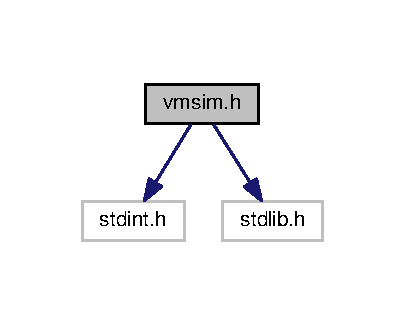
\includegraphics[width=195pt]{vmsim_8h__incl}
\end{center}
\end{figure}
This graph shows which files directly or indirectly include this file\+:\nopagebreak
\begin{figure}[H]
\begin{center}
\leavevmode
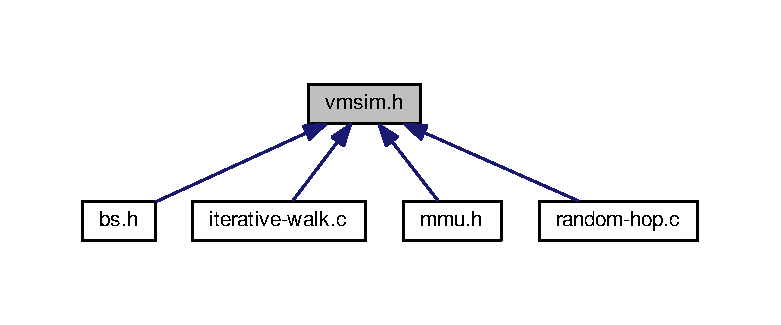
\includegraphics[width=350pt]{vmsim_8h__dep__incl}
\end{center}
\end{figure}
\subsection*{Macros}
\begin{DoxyCompactItemize}
\item 
\hypertarget{vmsim_8h_aea0cb1cd472958b65c6a163b409a22d5}{\#define {\bfseries P\+T\+E\+\_\+\+R\+E\+S\+I\+D\+E\+N\+T\+\_\+\+B\+I\+T}~0x1}\label{vmsim_8h_aea0cb1cd472958b65c6a163b409a22d5}

\item 
\hypertarget{vmsim_8h_a79cad0d5082cee52c764b431ce1d2dda}{\#define {\bfseries P\+T\+E\+\_\+\+R\+E\+F\+E\+R\+E\+N\+C\+E\+D\+\_\+\+B\+I\+T}~0x2}\label{vmsim_8h_a79cad0d5082cee52c764b431ce1d2dda}

\item 
\hypertarget{vmsim_8h_a0960c50fa38e76e51104b6413ec62fb4}{\#define {\bfseries P\+T\+E\+\_\+\+D\+I\+R\+T\+Y\+\_\+\+B\+I\+T}~0x4}\label{vmsim_8h_a0960c50fa38e76e51104b6413ec62fb4}

\end{DoxyCompactItemize}
\subsection*{Typedefs}
\begin{DoxyCompactItemize}
\item 
typedef uint32\+\_\+t \hyperlink{vmsim_8h_a1ad4b372d1694c5c19ee7ccada09d807}{vmsim\+\_\+addr\+\_\+t}
\item 
typedef uint32\+\_\+t \hyperlink{vmsim_8h_a673974423c805fd8f1c3a5212540ef08}{pt\+\_\+entry\+\_\+t}
\end{DoxyCompactItemize}
\subsection*{Functions}
\begin{DoxyCompactItemize}
\item 
void \hyperlink{vmsim_8h_ad6a84783f77b840cfa7e1100d58726b6}{vmsim\+\_\+read} (void $\ast$buffer, \hyperlink{vmsim_8h_a1ad4b372d1694c5c19ee7ccada09d807}{vmsim\+\_\+addr\+\_\+t} sim\+\_\+addr, size\+\_\+t size)
\begin{DoxyCompactList}\small\item\em Read data from the simulated space. \end{DoxyCompactList}\item 
void \hyperlink{vmsim_8h_a0c0214410981366e8ec1f218221380dc}{vmsim\+\_\+write} (void $\ast$buffer, \hyperlink{vmsim_8h_a1ad4b372d1694c5c19ee7ccada09d807}{vmsim\+\_\+addr\+\_\+t} sim\+\_\+addr, size\+\_\+t size)
\begin{DoxyCompactList}\small\item\em Write data into the simulated space. \end{DoxyCompactList}\item 
void \hyperlink{vmsim_8h_a3d4bf64eb67927a46562389b97988fc5}{vmsim\+\_\+read\+\_\+real} (void $\ast$buffer, \hyperlink{vmsim_8h_a1ad4b372d1694c5c19ee7ccada09d807}{vmsim\+\_\+addr\+\_\+t} real\+\_\+addr, size\+\_\+t size)
\begin{DoxyCompactList}\small\item\em Read data from the real space. \end{DoxyCompactList}\item 
void \hyperlink{vmsim_8h_ac3c6075c6e09967fe197e04de5094f52}{vmsim\+\_\+write\+\_\+real} (void $\ast$buffer, \hyperlink{vmsim_8h_a1ad4b372d1694c5c19ee7ccada09d807}{vmsim\+\_\+addr\+\_\+t} real\+\_\+addr, size\+\_\+t size)
\begin{DoxyCompactList}\small\item\em Write data into the real space. \end{DoxyCompactList}\item 
void \hyperlink{vmsim_8h_a2f2b0d73cdb718c73fbf3046dcaec0ca}{vmsim\+\_\+map\+\_\+fault} (\hyperlink{vmsim_8h_a1ad4b372d1694c5c19ee7ccada09d807}{vmsim\+\_\+addr\+\_\+t} sim\+\_\+addr)
\begin{DoxyCompactList}\small\item\em Create a new simulated-\/to-\/real mapping for a simulated address. \end{DoxyCompactList}\item 
\hyperlink{vmsim_8h_a1ad4b372d1694c5c19ee7ccada09d807}{vmsim\+\_\+addr\+\_\+t} \hyperlink{vmsim_8h_ad2d57f1bbe23c08a1cd4f10ed60ff3e0}{vmsim\+\_\+alloc} (size\+\_\+t size)
\begin{DoxyCompactList}\small\item\em Allocate simulated memory space. \end{DoxyCompactList}\item 
void \hyperlink{vmsim_8h_a49905ecd50563bbd6f5740023286acce}{vmsim\+\_\+free} (\hyperlink{vmsim_8h_a1ad4b372d1694c5c19ee7ccada09d807}{vmsim\+\_\+addr\+\_\+t} ptr)
\begin{DoxyCompactList}\small\item\em Deallocate simulated memory space. \end{DoxyCompactList}\end{DoxyCompactItemize}


\subsection{Detailed Description}
The interface for the {\ttfamily vmsim} library. 

\begin{DoxyAuthor}{Author}
Prof. Scott F. Kaplan 
\end{DoxyAuthor}
\begin{DoxyDate}{Date}
Fall 2018
\end{DoxyDate}
{\ttfamily vmsim} is a package that emulates a 32-\/bit virtual address space. It provides a {\itshape simulated address space} that is mapped onto a {\itshape real address space}. The real storage is created by the library, while a full 32-\/bit range of simulated addresses are mapped, on demand, onto that real storage space, which can be of any size. Space is created and mapped in 4 K\+B pages. Access to simulated storage is provided by the {\ttfamily vimsim\+\_\+read()} and {\ttfamily \hyperlink{vmsim_8h_a0c0214410981366e8ec1f218221380dc}{vmsim\+\_\+write()}} functions. 

\subsection{Typedef Documentation}
\hypertarget{vmsim_8h_a673974423c805fd8f1c3a5212540ef08}{\index{vmsim.\+h@{vmsim.\+h}!pt\+\_\+entry\+\_\+t@{pt\+\_\+entry\+\_\+t}}
\index{pt\+\_\+entry\+\_\+t@{pt\+\_\+entry\+\_\+t}!vmsim.\+h@{vmsim.\+h}}
\subsubsection[{pt\+\_\+entry\+\_\+t}]{\setlength{\rightskip}{0pt plus 5cm}typedef uint32\+\_\+t {\bf pt\+\_\+entry\+\_\+t}}}\label{vmsim_8h_a673974423c805fd8f1c3a5212540ef08}
A page table entry. \hypertarget{vmsim_8h_a1ad4b372d1694c5c19ee7ccada09d807}{\index{vmsim.\+h@{vmsim.\+h}!vmsim\+\_\+addr\+\_\+t@{vmsim\+\_\+addr\+\_\+t}}
\index{vmsim\+\_\+addr\+\_\+t@{vmsim\+\_\+addr\+\_\+t}!vmsim.\+h@{vmsim.\+h}}
\subsubsection[{vmsim\+\_\+addr\+\_\+t}]{\setlength{\rightskip}{0pt plus 5cm}typedef uint32\+\_\+t {\bf vmsim\+\_\+addr\+\_\+t}}}\label{vmsim_8h_a1ad4b372d1694c5c19ee7ccada09d807}
A simulated or real address within {\ttfamily vmsim}. 

\subsection{Function Documentation}
\hypertarget{vmsim_8h_ad2d57f1bbe23c08a1cd4f10ed60ff3e0}{\index{vmsim.\+h@{vmsim.\+h}!vmsim\+\_\+alloc@{vmsim\+\_\+alloc}}
\index{vmsim\+\_\+alloc@{vmsim\+\_\+alloc}!vmsim.\+h@{vmsim.\+h}}
\subsubsection[{vmsim\+\_\+alloc}]{\setlength{\rightskip}{0pt plus 5cm}{\bf vmsim\+\_\+addr\+\_\+t} vmsim\+\_\+alloc (
\begin{DoxyParamCaption}
\item[{size\+\_\+t}]{size}
\end{DoxyParamCaption}
)}}\label{vmsim_8h_ad2d57f1bbe23c08a1cd4f10ed60ff3e0}


Allocate simulated memory space. 


\begin{DoxyParams}{Parameters}
{\em size} & The number of bytes to allocate. \\
\hline
\end{DoxyParams}
\begin{DoxyReturn}{Returns}
the simulated address of the a block that is at least {\ttfamily size} bytes in length. 
\end{DoxyReturn}
\hypertarget{vmsim_8h_a49905ecd50563bbd6f5740023286acce}{\index{vmsim.\+h@{vmsim.\+h}!vmsim\+\_\+free@{vmsim\+\_\+free}}
\index{vmsim\+\_\+free@{vmsim\+\_\+free}!vmsim.\+h@{vmsim.\+h}}
\subsubsection[{vmsim\+\_\+free}]{\setlength{\rightskip}{0pt plus 5cm}void vmsim\+\_\+free (
\begin{DoxyParamCaption}
\item[{{\bf vmsim\+\_\+addr\+\_\+t}}]{ptr}
\end{DoxyParamCaption}
)}}\label{vmsim_8h_a49905ecd50563bbd6f5740023286acce}


Deallocate simulated memory space. 


\begin{DoxyParams}{Parameters}
{\em ptr} & The simulated address of a memory block allocated with {\ttfamily vmsim\+\_\+alloc}. \\
\hline
\end{DoxyParams}
\hypertarget{vmsim_8h_a2f2b0d73cdb718c73fbf3046dcaec0ca}{\index{vmsim.\+h@{vmsim.\+h}!vmsim\+\_\+map\+\_\+fault@{vmsim\+\_\+map\+\_\+fault}}
\index{vmsim\+\_\+map\+\_\+fault@{vmsim\+\_\+map\+\_\+fault}!vmsim.\+h@{vmsim.\+h}}
\subsubsection[{vmsim\+\_\+map\+\_\+fault}]{\setlength{\rightskip}{0pt plus 5cm}void vmsim\+\_\+map\+\_\+fault (
\begin{DoxyParamCaption}
\item[{{\bf vmsim\+\_\+addr\+\_\+t}}]{sim\+\_\+addr}
\end{DoxyParamCaption}
)}}\label{vmsim_8h_a2f2b0d73cdb718c73fbf3046dcaec0ca}


Create a new simulated-\/to-\/real mapping for a simulated address. 


\begin{DoxyParams}{Parameters}
{\em sim\+\_\+addr} & The simulated address for which to create the mapping.\\
\hline
\end{DoxyParams}
Called when the translation of a {\itshape simulated} address fails. When this function is done, a {\itshape real} page will back the {\itshape simulated} one that contains the given address, with the page tables appropriately updated.


\begin{DoxyParams}{Parameters}
{\em sim\+\_\+addr} & The {\itshape simulated} address for which address translation failed. \\
\hline
\end{DoxyParams}
\hypertarget{vmsim_8h_ad6a84783f77b840cfa7e1100d58726b6}{\index{vmsim.\+h@{vmsim.\+h}!vmsim\+\_\+read@{vmsim\+\_\+read}}
\index{vmsim\+\_\+read@{vmsim\+\_\+read}!vmsim.\+h@{vmsim.\+h}}
\subsubsection[{vmsim\+\_\+read}]{\setlength{\rightskip}{0pt plus 5cm}void vmsim\+\_\+read (
\begin{DoxyParamCaption}
\item[{void $\ast$}]{buffer, }
\item[{{\bf vmsim\+\_\+addr\+\_\+t}}]{sim\+\_\+addr, }
\item[{size\+\_\+t}]{size}
\end{DoxyParamCaption}
)}}\label{vmsim_8h_ad6a84783f77b840cfa7e1100d58726b6}


Read data from the simulated space. 


\begin{DoxyParams}{Parameters}
{\em buffer} & A pointer to a space into which to copy data from the simulated space. \\
\hline
{\em sim\+\_\+addr} & The simulated address from which to read the data. \\
\hline
{\em size} & The number of bytes to read, starting at the simulated address, into the buffer space. \\
\hline
\end{DoxyParams}
\hypertarget{vmsim_8h_a3d4bf64eb67927a46562389b97988fc5}{\index{vmsim.\+h@{vmsim.\+h}!vmsim\+\_\+read\+\_\+real@{vmsim\+\_\+read\+\_\+real}}
\index{vmsim\+\_\+read\+\_\+real@{vmsim\+\_\+read\+\_\+real}!vmsim.\+h@{vmsim.\+h}}
\subsubsection[{vmsim\+\_\+read\+\_\+real}]{\setlength{\rightskip}{0pt plus 5cm}void vmsim\+\_\+read\+\_\+real (
\begin{DoxyParamCaption}
\item[{void $\ast$}]{buffer, }
\item[{{\bf vmsim\+\_\+addr\+\_\+t}}]{real\+\_\+addr, }
\item[{size\+\_\+t}]{size}
\end{DoxyParamCaption}
)}}\label{vmsim_8h_a3d4bf64eb67927a46562389b97988fc5}


Read data from the real space. 


\begin{DoxyParams}{Parameters}
{\em buffer} & A pointer to a space into which to copy data from the real space. \\
\hline
{\em real\+\_\+addr} & The real address from which to read the data. \\
\hline
{\em size} & The number of bytes to read, starting at the real address, into the buffer space.\\
\hline
\end{DoxyParams}
This function is the analog to {\ttfamily \hyperlink{vmsim_8h_ad6a84783f77b840cfa7e1100d58726b6}{vmsim\+\_\+read()}}, except that the address given is the raw, {\itshape real} address, thus triggering no simulated-\/to-\/real mapping. \hypertarget{vmsim_8h_a0c0214410981366e8ec1f218221380dc}{\index{vmsim.\+h@{vmsim.\+h}!vmsim\+\_\+write@{vmsim\+\_\+write}}
\index{vmsim\+\_\+write@{vmsim\+\_\+write}!vmsim.\+h@{vmsim.\+h}}
\subsubsection[{vmsim\+\_\+write}]{\setlength{\rightskip}{0pt plus 5cm}void vmsim\+\_\+write (
\begin{DoxyParamCaption}
\item[{void $\ast$}]{buffer, }
\item[{{\bf vmsim\+\_\+addr\+\_\+t}}]{sim\+\_\+addr, }
\item[{size\+\_\+t}]{size}
\end{DoxyParamCaption}
)}}\label{vmsim_8h_a0c0214410981366e8ec1f218221380dc}


Write data into the simulated space. 


\begin{DoxyParams}{Parameters}
{\em buffer} & A pointer to a space from which to copy data into the simulated space. \\
\hline
{\em sim\+\_\+addr} & The simulated address into which to write the data. \\
\hline
{\em size} & The number of bytes to write, starting at the simulated address, from the buffer space. \\
\hline
\end{DoxyParams}
\hypertarget{vmsim_8h_ac3c6075c6e09967fe197e04de5094f52}{\index{vmsim.\+h@{vmsim.\+h}!vmsim\+\_\+write\+\_\+real@{vmsim\+\_\+write\+\_\+real}}
\index{vmsim\+\_\+write\+\_\+real@{vmsim\+\_\+write\+\_\+real}!vmsim.\+h@{vmsim.\+h}}
\subsubsection[{vmsim\+\_\+write\+\_\+real}]{\setlength{\rightskip}{0pt plus 5cm}void vmsim\+\_\+write\+\_\+real (
\begin{DoxyParamCaption}
\item[{void $\ast$}]{buffer, }
\item[{{\bf vmsim\+\_\+addr\+\_\+t}}]{real\+\_\+addr, }
\item[{size\+\_\+t}]{size}
\end{DoxyParamCaption}
)}}\label{vmsim_8h_ac3c6075c6e09967fe197e04de5094f52}


Write data into the real space. 


\begin{DoxyParams}{Parameters}
{\em buffer} & A pointer to a space from which to copy data into the real space. \\
\hline
{\em real\+\_\+addr} & The real address into which to write the data. \\
\hline
{\em size} & The number of bytes to write, starting at the real address, from the buffer space.\\
\hline
\end{DoxyParams}
This function is the analog to {\ttfamily \hyperlink{vmsim_8h_a0c0214410981366e8ec1f218221380dc}{vmsim\+\_\+write()}}, except that the address given is the raw, {\itshape real} address, thus triggering no simulated-\/to-\/real mapping. 
%--- End generated contents ---

% Index
\newpage
\phantomsection
\addcontentsline{toc}{chapter}{Index}
\printindex

\end{document}
